\documentclass[a4paper]{article}

% Packages.
\usepackage{amsmath}
\usepackage{amsthm}
\usepackage[answerdelayed]{exercise}
\usepackage[usenames,dvipsnames]{color}

% Definitions.
\theoremstyle{definition}
\newtheorem{definition}{Definition}

\renewcommand{\ExerciseHeader}{\vspace{7mm}\par\noindent\textbf{\large
\ExerciseName\ \ExerciseHeaderNB\ExerciseHeaderTitle
\ExerciseHeaderOrigin}\par}

\renewcommand{\AnswerHeader}{\par\noindent\textbf{
Answer of \ExerciseName\ \ExerciseHeaderNB}\par}

% Options.


\title{The Wilcoxon test}
\author{Guillaume Filion}
\usepackage{Sweave}
\begin{document}
\maketitle


%% The problem %%
\section{The problem}

In 1980, John F. Laszlo studied the role of 2-chlorobenzoate on the
eclosion time in larch bud moth. He obtained the following values (in
hours):

\begin{Schunk}
\begin{Sinput}
> non_treated <- c(48.90, 20.98, 52.07, 25.57, 24.01, 51.50, 26.40);
> treated <- c(49.88, 44.00, 24.79, 45.93, 48.20, 26.51, 21.27);
\end{Sinput}
\end{Schunk}

\begin{Exercise}
Can we assume that the eclosion time is Gaussian? Can we apply the
Central Limit Theorem?
\end{Exercise}
\begin{Answer}
No: the data is bimodal (eclosion time depends on the hour of the
day). No: the datasets are too small.
\end{Answer}


%% The null hypothesis %%
\section{The null hypothesis}

What can we do if we really cannot assume that the variables are Gaussian
and the sample size is too small to apply the Central Limit Theorem
(roughly $n < 30$)? The $t$ test is no longer a good option.

We need to find another way to measure the differences between samples.
If working with absolute differences does not work, we can try relative
differences. After all, if all the values of a sample were higher than the
values of the other, we would probably conclude that there is a difference,
even if those numbers are close.

\begin{Exercise}
Together, propose a test based on relative differences. Formulate the
null and the alternative hypotheses and design the test statistic.
\end{Exercise}
\begin{Answer}
The idea is to work with the ranks of the values. The null hypothesis
of the test is composed of a single statement:
\begin{enumerate}
\item
Sampling is IID across samples.
\end{enumerate}
The null hypothesis is very general, so you might think that we have
found the perfect test. However, the alternative hypothesis is somewhat
restrictive:
\begin{enumerate}
\item
Sampling is IID within each sample.
\item
Distributions differ by a `horizontal' shift.
\end{enumerate}
Thus, not every difference in distribution will lead to the rejection
of the null hypothesis.
A good test statistic to choose for this approach is the mean of the
ranks of the values of the first sample. For example, if we have two
samples $(1.2, 10.3)$ and $(3.4, 5.0, 17.1)$, the test statistic is
$(1+4)/2$. We will call this statistic $U$.

However, the literature is not unanimous on which statistic to
use, several others are available. The statistic used in \texttt{R},
is $W$. If the two samples are denoted $(x_1, ..., x_n)$ and
$(y_1, ..., y_m)$, $W$ is the number of pairs $(x_i, y_j)$
for which $x_i \geq y_j$. In the previous example, the statistic is 2.
\end{Answer}


%% The test statistic %%
\section{Computing the test statistic}

We have a test statistic $U$ based on the ranks. We need to
be able to extract the ranks from a collection of samples and
compute the test statistic.

\begin{Exercise}
Compute the ranks of the sample $(2.6, 8.2, 1.3)$.
\par\noindent\textcolor{Blue}{\textbf{Hint:} Use the function
\texttt{rank}.}
\end{Exercise}
\begin{Answer}
\begin{Schunk}
\begin{Sinput}
> rank(c(2.6, 8.2, 1.3));
\end{Sinput}
\begin{Soutput}
[1] 2 3 1
\end{Soutput}
\end{Schunk}
\end{Answer}

\begin{Exercise}
We have to choose which ranks to give in case the values are equal.
What does the function \texttt{rank} do with ties by default?
\end{Exercise}
\begin{Answer}
It gives the average rank.
\end{Answer}

\begin{Exercise}
Write a function that computes the $U$ statistic (of the first
of two samples). Use it to compute the $U$ statistic of the
data.
\end{Exercise}
\begin{Answer}
\begin{Schunk}
\begin{Sinput}
> # Didactic version:
> U <- function(x, y) { 
+    allranks <- rank(c(x,y));
+    ranksx <- allranks[1:length(x)];
+    return (mean(ranksx));
+ }
> # What I would write:
> U <- function(x,y) {
+    # Return the U statistic for sample x.
+    mean(rank(c(x,y))[1:length(x)]);
+ }
> U.obs <- U(treated, non_treated);
> U.obs;
\end{Sinput}
\begin{Soutput}
[1] 7.428571
\end{Soutput}
\end{Schunk}
\end{Answer}


%% The distribution of U %%
\section{The distribution of $U$}

We are now faced with a problem: what distribution are we going to
use to generate samples under the null hypothesis in order to compute
the $U$ statistic?

The beauty of this approach is that \textbf{it does not matter!}
Indeed, if ranks are sampled from the exact same distribution,
it is like picking the first 14 numbers and assigning 7
at random to sample 1 and the 7 other to sample 2.
We will verify this now.

\begin{Exercise}
Generate 10,000 values of $U$ obtained from 2 standard Gaussian samples
of size 7. Store the result in a vector \texttt{U.Gaussian}.
\par\noindent\textcolor{Blue}{\textbf{Hint:} Use a \texttt{for} loop.}
\end{Exercise}
\begin{Answer}
\begin{Schunk}
\begin{Sinput}
> U.Gaussian <- rep(NA, 10000);
> for (i in 1:10000) {
+    U.Gaussian[i] <- U(rnorm(7), rnorm(7));
+ }
\end{Sinput}
\end{Schunk}
\end{Answer}

\begin{Exercise}
Do the same with 2 exponential samples and store the result in a vector
\texttt{U.exp}. Then do the same with 2 uniform samples and store the
result in a vector \texttt{U.unif}. Finally, overlay the density
distributions of those computations of $U$.
\par\noindent\textcolor{Blue}{\textbf{Hint:} Use \texttt{rexp} and
\texttt{runif}.}
\par\noindent\textcolor{BrickRed}{\textbf{For the aces:} what happens
to the $U$ statistic if samples differ only through their spread?
Is the Wilcoxon test robust to the assumption that both distributions
must have the same spread?}
\end{Exercise}
\begin{Answer}
\begin{Schunk}
\begin{Sinput}
> U.exp <- rep(NA, 10000);
> U.unif <- rep(NA, 10000);
> for (i in 1:10000) {
+    U.exp[i] <- U(rexp(7), rexp(7));
+    U.unif[i] <- U(runif(7), runif(7));
+ }
> plot(density(U.Gaussian), main="Density plots", xlab="Value");
> lines(density(U.exp), col=2);
> lines(density(U.unif), col=3);
> legend(x="topright", legend=c("Gaussian", "Exponential", "Uniform"),
+    lwd=1, col=c(1,2,3));
\end{Sinput}
\end{Schunk}
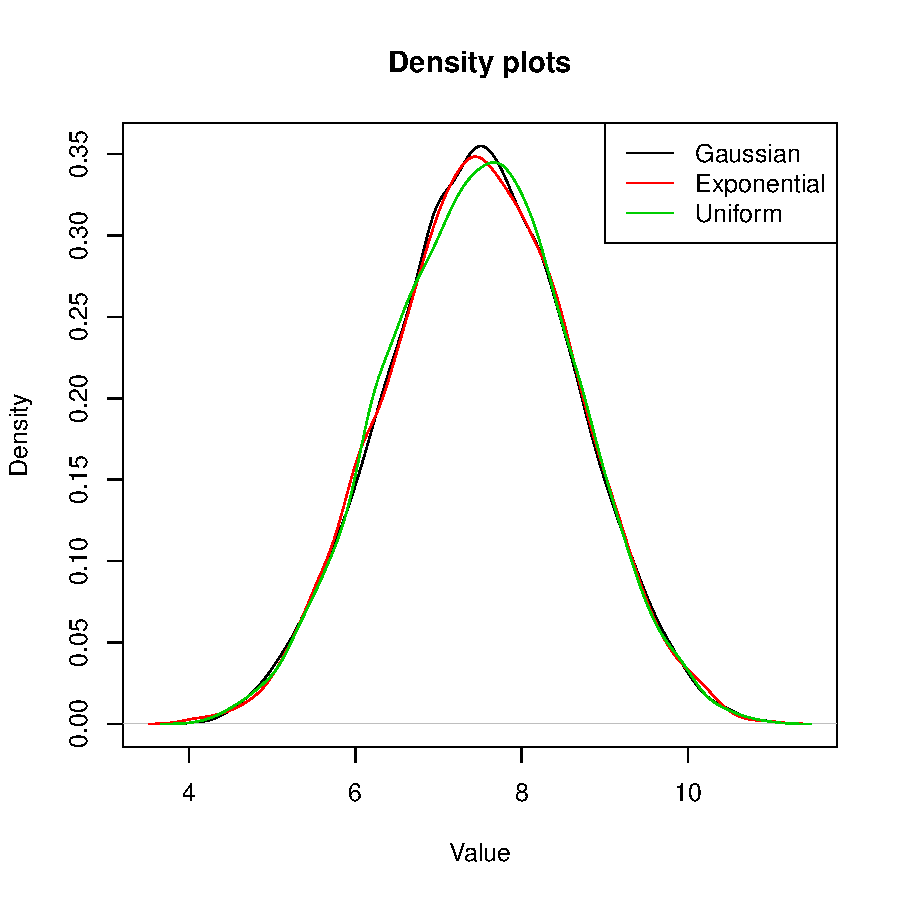
\includegraphics{wilcoxon-005}
\end{Answer}

%% The decision rule %%
\section{The decision rule}

Now we need a decision rule. We will use the same approach as
for the $t$ test, \textit{i.e.} define a rejection region at level
0.05, symmetric and away from the central bulk of points. The
difference is that the distribution of $U$ is not centered,
so we need to know this central value.

\begin{Exercise}
What is the exact expected value of $U$?
\end{Exercise}
\begin{Answer}
The sum of the ranks of the first sample ($\tilde{U}_1$) and the
second sample ($\tilde{U}_2$) is always $1+2+...+14 = 105$.
Because of symmetry, the expected values of $\tilde{U}_1$ and
$\tilde{U}_2$ must be equal.
\begin{equation*}
   E\{\tilde{U}_1 + \tilde{U}_2\} = 2 E\{\tilde{U}_1\} = 105 \mbox{, so }
   E \{\tilde{U}_1\} = 105/2 = 52.5
\end{equation*}
By definition, the statistic $U$ is $\tilde{U}_1/7$ So $E{U}=7.5$.
\end{Answer}

\begin{Exercise}
Get the approximate limits of the rejection region and finish the
test. Estimate the p-value and compare your results with the output
of \texttt{wilcox.test}.
\end{Exercise}
\begin{Answer}
\begin{Schunk}
\begin{Sinput}
> # Get an estimate of the acceptance region.
> quantile(U.Gaussian, probs=c(0.025, 0.975));
\end{Sinput}
\begin{Soutput}
    2.5%    97.5% 
5.285714 9.714286 
\end{Soutput}
\begin{Sinput}
> # The null hypothesis is accepted.
> # To check the p-value, we center and symmetrize the
> # statistic U statistic.
> mean(abs(U.Gaussian - 7.5) >= abs(U.obs - 7.5));
\end{Sinput}
\begin{Soutput}
[1] 1
\end{Soutput}
\begin{Sinput}
> wilcox.test(treated, non_treated);
\end{Sinput}
\begin{Soutput}
	Wilcoxon rank sum test

data:  treated and non_treated 
W = 24, p-value = 1
alternative hypothesis: true location shift is not equal to 0 
\end{Soutput}
\end{Schunk}
\end{Answer}

\cleardoublepage
\shipoutAnswer
\end{document}
